\section{Modelo de Referência}
%Apresentação dos conceitos de BI
O modelo de referência idealizado e implementado no TRE-RN é composto por componentes de \textit{software} capazes de realizar as atividades referentes ao processo de desenvolvimento de aplicações de \textit{business intelligence}, sendo elas: ETL, DW e visualização.
A etapa de ETL (\textit{Extract, Transform and Load}), corresponde ao processo de extração, transformação e carga dos dados oriundos das diversas fontes de negócio em um repositório de dados dedicado ao processo de análise. Os dados resultantes da atividade de ETL devem encontrar-se integrados e modelados em um formato mais adequado a carga imposta pelo processo analítico. 
Esse repositório mencionado é exatamente a segunda etapa de um processo BI, denominado \textit{Data Warehouse}, que em traducão literal significa armazém de dados, e consiste no armazenamento dos dados produzidos pelo processo anterior.
De posse dos dados já tratados e persistidos em um \textit{Data Warehouse}, inicia-se a etapa de visualização dos dados, que consiste no desenvolvimento de painéis visuais responsáveis por apresentar as informações necessárias para a tomada de decisão de negócio.

%Breve descrição do modelo de referência
As atividades descritas acima, são executadas no modelo de referência pelos seguintes componentes de \textit{software}: \textit{Pentaho Data Integration}, realizando as atividades de ETL, PostgreSQL, atuando como um DW, e o \textit{Metabase} sendo o componente onde são desenvolvidos e apresentados os painéis gráficos. O modelo de referência é ilustrado na Figura \ref{fig:modelo_referencia}

% Imagem da arquitetura do modelo de referência
\begin{figure}[htp]
   \centering
    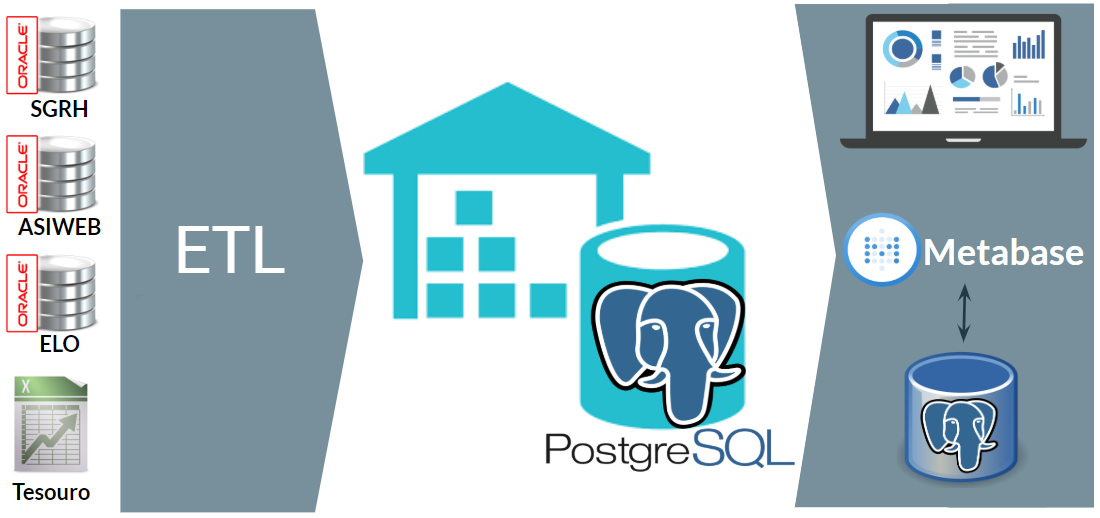
\includegraphics[width=8cm]{Imagens/Arq_TRE}
    \caption{Arquitetura de BI no TRE-RN.}
    \label{fig:modelo_referencia}
\end{figure} 

Conforme indicado anteriormente, este trabalho demonstra a implantação de um processo de orquestação de multiplas instâncias para garantir a escalabilidade sob demanda, inicialmente, aplicado na camada de visualização, ou seja, do \textit{Metabase}. Para que possamos realizar o objetivo exposto, precisamos descrever melhor a arquitetura do componente em questão, bem como, as demais ferramentas que serão utilizadas. 

\subsection{Ferramentas}

\subsubsection{\textit{Docker}}

Conforme descrito em sua documentação oficial \cite{dockerDoc}, o \textit{Docker} é uma plataforma de \textit{software} aberto voltada para o desenvolvimento, entrega e execução de aplicações isoladamente. Esta unidade isolada, resultante do uso do \textit{Docker}, é denominada como container. Os containeres atendem basicamente os mesmos propósito das máquinas virtuais (VMs) e são executados sobre uma máquina física ou até mesmo virtual. No entento, diferente das VMs, os containeres não são executados sobre um virtualizador, mas diretamente no \textit{kernel} da máquina hospedeira, o que lhes garante uma estrutura mais enxuta.

Essa tecnologia já é utilizada em aplicações que suportam a atividade do TRE-RN, sejam elas desenvolvidas pelo próprio Tribunal ou adquirida de terceiros. Logo, por ter o corpo técnico de servidores fortemente capacitados na manutenção e utilização de \textit{Docker}, a utilização desta ferramenta foi sugerida como base para o modelo de referência desde o início das atividades.

\subsubsection{PostgreSQL}

Outra ferramenta relavante para o projeto do modelo de refência é o PostgreSQL. Utilizado como DW e como repositório dos metadados do \textit{Metabase}, o PostgreSQL é um Sistema de Gerencimento de Banco de Dados (SGBD) de código aberto desenvolvimento, inicialmente, pela Universidade da Califórnia, conforme apresentado pela documentação oficial da ferramenta \cite{postgresDoc}.

A escolha do PostgreSQl foi uma sugestão do TRE-RN visto o longo histórico de utilização da ferramenta pelo Tribunal em projetos extremamente relevantes. Por exemplo, este SGBD é responsável pela gestão dos dados oriundos do sistema de Processo Judicial Eletrônico (PJe), onde tramitam, atualmente, todos os processos de segundo grau da justiça eleitoral do Rio Grande do Norta.

Assim como com o \textit{Docker}, o corpo técnico do Tribunal possui a capacitação mais do que necessária para implantação de manutenção de instância de PostgreSQL. 

\subsubsection{Metabase}

O \textit{Metabase} é uma aplicação \textit{web}, desenvolvida e mantida por uma comunidade aberta, que consiste em uma aplicação \textit{backend} que contém uma API REST, bem como os códigos para comunicação com os bancos de dados e realizar o processamento dos resultados das consultas, e uma aplicação \textit{frontend} de página única (\textit{Single Page Application}) responsável pelas interfaces de usuário do sistema, conforme descreve o guia do desenvolvedor \cite{metabaseeevguide}. Vale ressaltar que ambos o \textit{backend} quanto o \textit{frontend} da aplicação são encapsudos em um único pacote de \textit{software}, que na realidade do TRE é hospedado por um container Docker.
Além dos sub componentes já explicitados, o \textit{Metabase} depende um sistema de gerenciamento de banco de dados (SGBD) que irá armazenar e servir os metadados da própria aplicação. A configuração definida pelo corpo técnico do Tribunal foi a utilização do PostgreSQL para servir a este propósito, dado \textit{expertise} previamente adquirida na implantação e manuteção deste SGBD. A Figura \ref{fig:arq_metabase} ilustra a configuração descrita acima. 

% Imagem da arquitetura do metabase
\begin{figure}[htp]
   \centering
    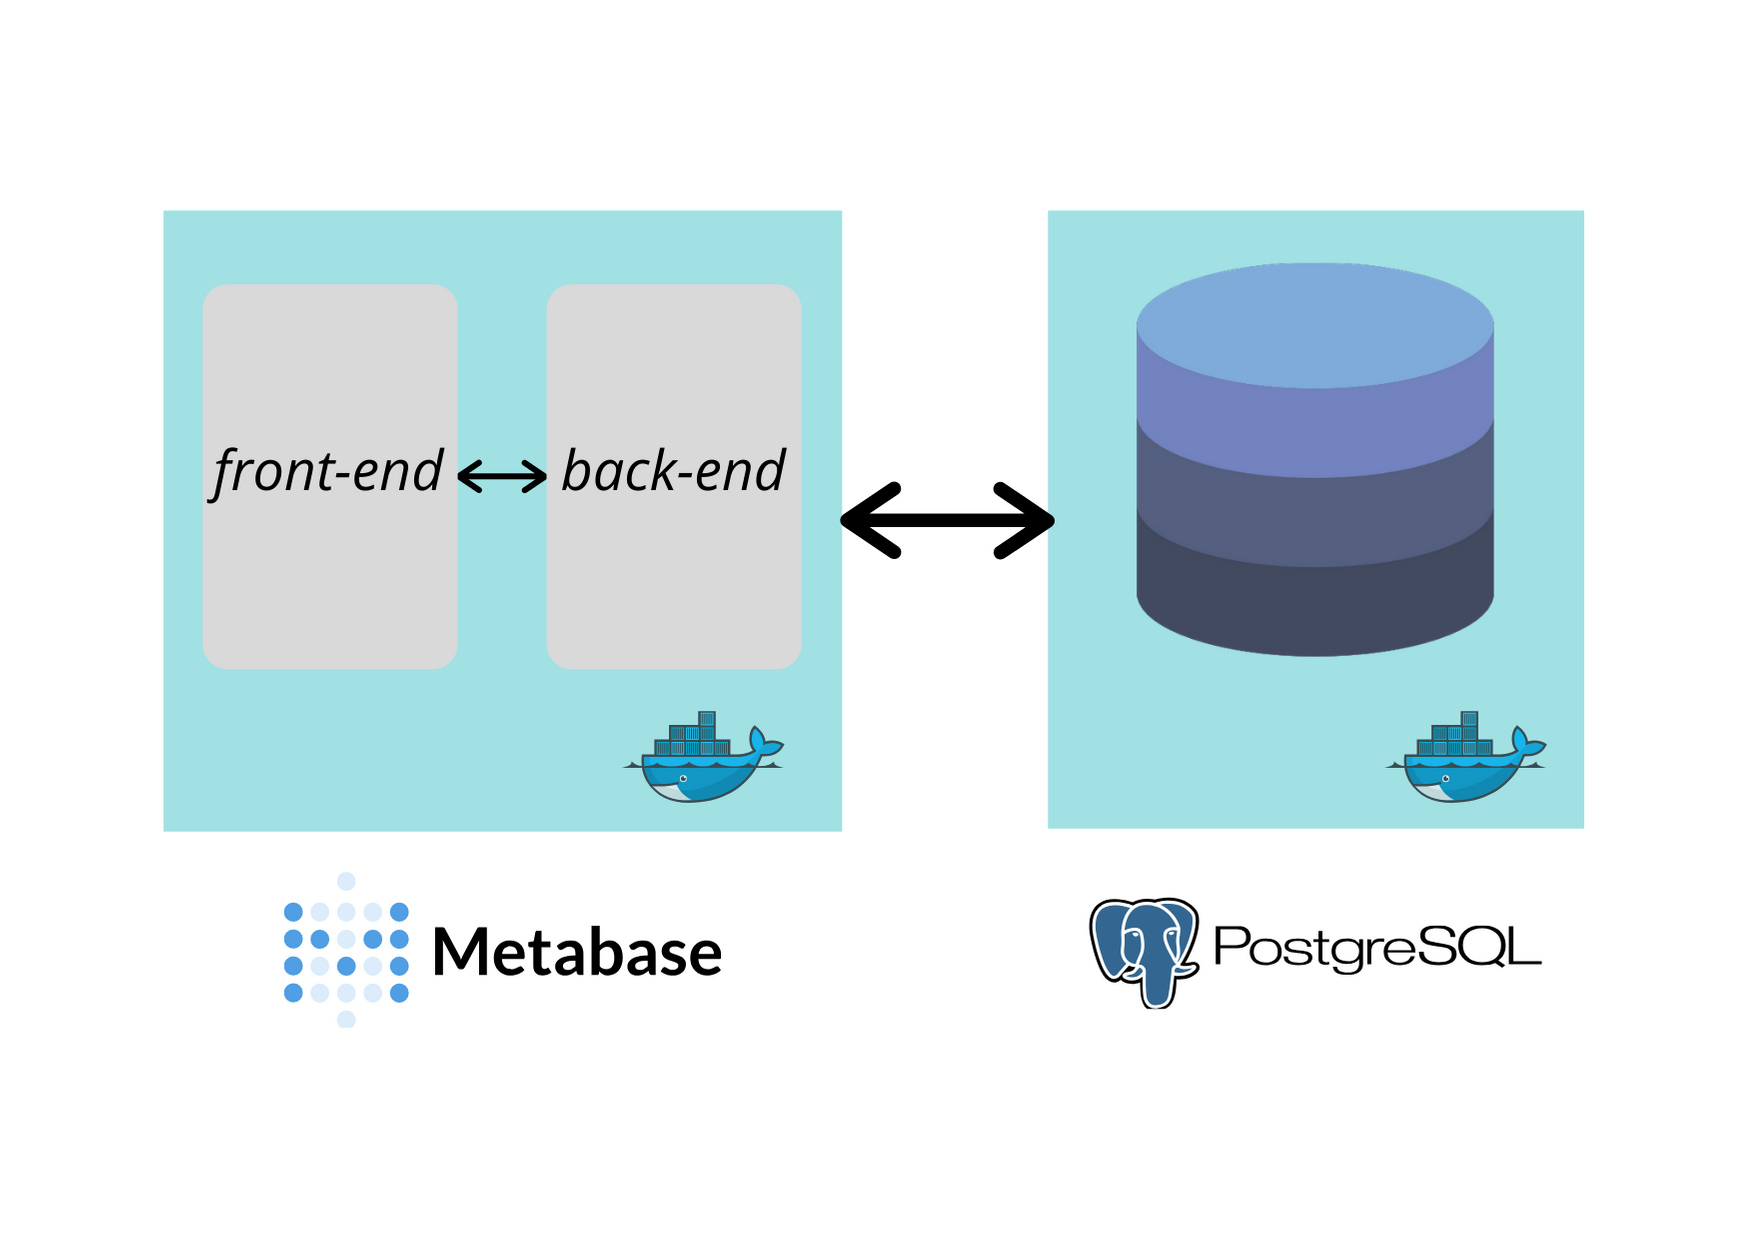
\includegraphics[width=8cm]{Imagens/Arq_Metabase}
    \caption{Arquitetura do \textit{Metabase}.}
    \label{fig:arq_metabase}
\end{figure} 


